\chapter{Automação Veicular}
\label{cap:automacao_veicular}

A automação veicular faz um extenso uso de componentes eletrônicos em seus sistemas. Nos tópicos que seguem serão abordados os domínios eletrônicos de funcionamento em veículos, seus meios de comunicação, unidades de controle e engenharia de software automotivo.

\section{Transição da Mecânica para Eletrônica}

De acordo com \citeonline{BoschBiblia}, os motivos para evolução automotiva variam entre ganhos de desempenho e segurança, barateamento de sistemas sem perda de qualidade e a adequação as leis de trânsito e meio-ambiente. 

Contudo, independente da motivação, é notável que há cada vez mais a adoção de sistemas eletrônicos embarcados. A \reffig{cap2_car_evolution} ilustra veículos de eras diferentes, a primeira dotada de recursos mecânicos, enquanto que a segunda destaca as centrais eletrônicas, as quais vem aumentando em número a cada ano que passa.

\begin{figure}[htb]
	\centering
	\caption{Evolução dos componentes eletrônicos.}
	\subfigure[1950]{\label{fig:cap2_car_ecus_fusca}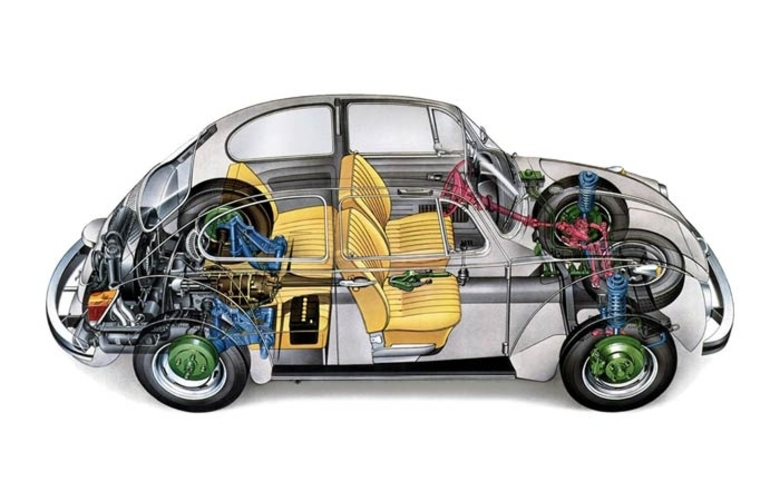
\includegraphics[width=0.45\textwidth]{cap2_car_ecus_fusca.png}}
	\subfigure[2000]{\label{fig:cap2_car_ecus_mercedes}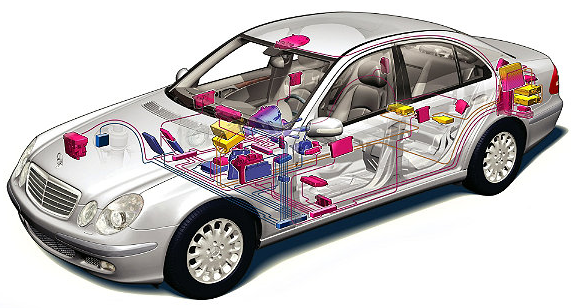
\includegraphics[width=0.45\textwidth]{cap2_car_ecus_mercedes.png}}
	Extraido de: \citeonline{Fusca} e \citeonline{Mercedes}.
	\label{fig:cap2_car_evolution}
\end{figure}

Nos dias de hoje, recursos como injeção eletrônica e freios \criarSigla[Sistema de Anti-Bloqueio]{Antiblockier-Bremssystem}{ABS} são exigências para que um novo modelo de carro possa entrar em circulação.

O crescente uso de recursos eletrônicos demanda também que os mesmos possam se comunicar e cooperar entre si, para que o máximo de desempenho possa ser extraído dos sistemas. Neste caso, os domínios funcionais auxiliam na classificação e responsabilidade destes sistemas.

\section{Domínios Funcionais de uma Arquitetura Veicular}

De modo a facilitar a classificação e identificação de sistemas eletrônicos que compõem um veículo, historicamente, foram estabelecidos cinco domínios de funcionalidade na arquitetura veicular, sendo eles o \emph{Trem de Força}, \emph{Chassi}, \emph{Corpo}, \criarSigla{Interface Homem-Máquina}{IHM} e \emph{Telemática} \cite{Auto:Lion2008}.

Com o avanço das últimas décadas, recursos veiculares pertencentes a estes domínios que até então eram implementados via sistemas mecânicos e elétricos puderam ser substituídos por elementos da eletrônica, agregando confiabilidade, segurança e, em alguns casos, possibilitando o atendimento de requisitos que antes eram inviáveis de implementação.

Nas demais subseções, serão apresentados em mais detalhes cada um dos domínios funcionais e serão levantados exemplos de como eles se beneficiaram nos últimos anos com o uso de microeletrônicos e microprocessadores.

\subsection{Trem de Força}

O domínio do trem de força está relacionado aos sistemas que participam na propulsão longitudinal de um veículo. Conforme pode ser observado pela \reffig{cap2_power_train}, estes sistemas são compreendidos pelo \emph{motor}, \emph{transmissão} e demais componentes subsidiários, como o \emph{trem de rodagem}\footnote{Drive Train, no inglês.}.

\figura{cap2_power_train}{Trem de força de um veículo automotivo}{7cm}{Auto:Lion2008}

Os sistemas presentes neste domínio buscam otimizar componentes para condução, conforto, economia de combustível, dentre outros. Há uma grande quantidade de sistemas embarcados vinculados principalmente ao motor, onde desde $1939$ a empresa Bosch já fazia pesquisas sobre o gerenciamento eletrônico de motores \cite{BoschHistory}.

Um sistema bastante conhecido no ramo automobilístico, e que veio a substituir completamente o uso de carburadores, é a injeção eletrônica, implementado comercialmente pela primeira vez pela Bendix Corporation, em $1958$\footnote{Na época batizado de \emph{Electrojector} pela empresa.}\cite{Electrojector}. Este sistema é responsável pela injeção de combustível dentro do motor e controla as quantidades e proporção entre ar e comburente, bem como a produção da centelha pelas velas de ignição. O controle de tempos e proporções parte de uma \criarSigla[Unidade de Controle Eletrônica]{Eletronic Control Unit}{ECU}, componente o qual será discutido em maior detalhes na \reftop{ecu}. A \reffig{cap2_eletronic_injection} apresenta um modelo com os bicos injetores e sua respectiva ECU.

\figura{cap2_eletronic_injection}{Injeção Eletrônica e ECU}{7cm}{BoschInjecao}

%Sistemas embarcados localizados próximos ao motor precisam ser resistentes a interferências, como a alta temperatura, por exemplo. Algumas das outras características desejáveis para sistemas embarcados neste domínio são:
%
%\begin{itemize}
%	\item Suporte a restrições temporais rígidas, descrito em mais detalhes na \reftop{tempo_real};
%	\item Componentes discretos;
%	\item Alta amostragem de sinais, na casa dos nanosegundos\footnote{Para amostragem de dados no motor.}.
%\end{itemize}

\subsection{Chassi}

Os elementos que compõem o \emph{Chassi} tem por objetivo controlar a interação do veículo com o ambiente ao qual ele irá circular. Isto é alcançado através de leituras e atuações nas rodas, suspensões, sistemas de freio, direção, aceleração, dentre outros. Em carros mais modernos, também são levados em conta as condições da estrada, velocidade do vento, situação do clima e outros fatores externos ao veículo.

Dos sistemas que compõem este domínio, podem ser citados os de ABS, \criarSigla[Programa Eletrônico de Estabilidade]{Electronic Stability Program}{ESP}, \criarSigla[Controle de Estabilidade Automática]{Automatic Stability Control}{ASP} e o \criarSigla[Tração nas Quatro Rodas]{Four-Wheel Drive}{4WD}. A \reffig{cap2_chassi_abs} apresenta uma ilustração dos componentes do ABS.

\figura{cap2_chassi_abs}{Componentes do sistema de ABS}{7cm}{Injecao}

Como o domínio do \emph{chassi} tem por objetivo a segurança dos passageiros e do próprio veículo, seus sistemas utilizam recursos de alta qualidade e o mesmo é tratado como um setor crítico. Características desejáveis são similares a do \emph{trem de força}, fazendo uso de uma técnica adicional de segurança chamada de \emph{X-by-Wire}\footnote{Traduzico do inglês como \emph{X-por-fio}}. Este método consiste em manter um sistema mecânico (ergo, o \emph{"por fio"} do nome) redundante ao eletrônico. Historicamente, o sistema mecânico é o sistema original, sendo mantido apenas por questões de segurança.

\subsection{Corpo}

O domínio do \emph{Corpo} do veículo incluí os demais sistemas que não estão relacionados ao controle de suas dinâmicas. Mecanismos como limpadores de vidro, faróis, portas e janelas, assentos e retrovisores hoje em dia são controlados diretamente por sistemas baseados em software. A \reffig{cap2_body_systems} provê uma ilustração de alguns destes sistemas e sua localização no veículo.

\figura{cap2_body_systems}{Sistemas pertencentes ao domínio do \emph{corpo}. Em destaque o mecanismo de abertura e fechamento dos vidros}{7cm}{body_system}

De uma maneira geral, estes sistemas, embora necessários para o devido funcionamento do veículo e conforto dos passageiros, não representam um fator crítico de proteção para o usuário, salvo alguns sistemas de segurança quanto ao controle de acesso do veículo.

Este domínio geralmente envolve a comunicação de diversas funções entre si, o que, consequentemente, gera uma arquitetura complexa distribuída. Desta necessidade emerge o conceito de subsistemas baseados em redes de sensores-atuadores de baixo custo.

Um sistema de controle para portas, por exemplo, poderia utilizar uma ECU principal para realizar as operações da porta do motorista (trancar/destrancar a porta, fechar/abrir janela, ajustar o banco). Esta ECU se comunicaria com as ECUs da trava, janela e banco por uma rede \criarSigla[Rede Local Interconectada]{Local Interconnect Network}{LIN}\refcap{rede_lin} de baixo custo. Como uma operação de trancar/destrancar uma porta pode influenciar nas outras, todas as ECUs das portas estariam conectadas por uma rede \criarSigla[Área de Rede Controladora]{Controller Area Network}{CAN}\refcap{rede_can}, assim como com o painel, afim de indicar o estado das portas. A \reffig{cap2_body_doors} apresenta uma ilustração destas interações.

\figura{cap2_body_doors}{Comunicação de uma ECU principal com as demais}{7cm}{Auto:Lion2008}

\subsection{IHM e Telemáticos}

O domínio da \emph{interface homem-máquina} governa a iteração do condutor e passageiros com as várias funções embarcadas do veículo. Resultados que podem ser apresentados pela IHM são:

\begin{itemize}
	\item Estados do Veículo: velocidade, nível do óleo, situação das portas, estado das luzes;
	\item Estado de um dispositivo multimídia: rádio sintonizada, controle de volume;
	\item Reposta a uma requisição: visualização de um mapa no sistema de navegação.
\end{itemize}

Sistemas embarcados deste domínio geralmente estão instalados no painel de um veículo, conforme ilustração da \reffig{cap2_hmi_panel}.

\figura{cap2_hmi_panel}{Painel de um carro}{7cm}{hmi_panel}

O domínio da \emph{telemática}, em contraste à IHM, governa a troca de informações entre veículos ou entre o veículo e infraestruturas da estrada.

Exemplos de sistemas deste domínio são os coletores automáticos de tarifas para pedágios, no qual o carro pode passar por uma via sem precisar parar para realizar o pagamento em dinheiro. Outras aplicações incluem a comunicação com serviços de trânsito, os quais podem indicar a situação em uma rodovia, como acidentes ou trânsito intenso.

Uma das transições que a área está passando atualmente é no desenvolvimento de carros inteligentes, capazes de detectar riscos ao motorista e, até mesmo, dirigir automaticamente, sem que haja a necessidade de intervenção do condutor humano. Empresas como a Google e a Tesla estão com soluções comerciais em fase de avaliação no mercado.

A \reffig{cap2_telematic_smart} ilustra a visão do veículo para com seus meios externos, identificando veículos e limites de velocidades.

\figura{cap2_telematic_smart}{Visão dos sistemas de um carro automático}{7cm}{telematic_smart}

Ambos os domínios estão se aproximando cada vez mais do conceito de Internet das Coisas, onde os veículos serão um dos grandes beneficiados desta integração, devido aos novos tipos de serviços e informações que serão trocadas por eles \cite{IoT}.

\section{Protocolos de Comunicação Automotivos}

Devido a grande quantidade de componentes que necessitam trocar informações em um veículo, é imperativo que existam meios de comunicação padronizados e que atendam aos requisitos dos sistemas, como taxa de transmissão e segurança. Os protocolos de comunicação permitem que estas integrações sejam realizáveis com relativa facilidade.

Embora mais complexas, é comum o uso de redes distribuídas em veículos automotivos, onde mais de um protocolo de comunicação são empregados.

%Alguns destes protocolos atendem ao padrão \emph{ISO 7498}, utilizando sete camadas para comunicação, cada qual com uma responsabilidade. Resumidamente, as camadas deste protocolo são:
%\begin{itemize}
%	\item \textbf{Camada 7}: Aplicação;
%	\item \textbf{Camada 6}: Apresentação;
%	\item \textbf{Camada 5}: Sessão;
%	\item \textbf{Camada 4}: Transporte;
%	\item \textbf{Camada 3}: Rede;
%	\item \textbf{Camada 2}: Enlace de Dados;
%	\item \textbf{Camada 1}: Física;
%\end{itemize}

\subsection{Protocolos Automotivos}

Existem diversos protocolos automotivos, os quais estão listados em \citeonline{EletroEmb} e devidamente identificados quanto a fabricante, aplicação, tipo de barramento, dentre outros quesitos.

A classificação destes é feita por meio de grupos, os quais definem a taxa de transmissão e/ou aplicação dos mesmos. A \reftab{cap2_protocolos} lista estes grupos de uma maneira resumida.

\begin{table}[h]
	\centering
	\caption{Grupos de Protocolos.}
	\label{tab:cap2_protocolos}
	\begin{tabular}{ccc}
		Grupo         & Caracteristicas \& Uso                                                    & Protocólos                 \\ \hline \hline
		Classe A      & \begin{tabular}[c]{@{}l@{}}Conforto\\ 10Kbps\end{tabular}                 & SINEBUS, $I^2C$, SAE, LIN  \\ \hline
		Classe B      & \begin{tabular}[c]{@{}l@{}}Entretenimento\\ 10Kbps a 125Kbps\end{tabular} & CAN 2.0, Class 2, SCP, PCI \\ \hline
		Classe C      & \begin{tabular}[c]{@{}l@{}}Segurança\\ 125Kbps a 1Mbks\end{tabular}       & CAN 2.0, ISO, SAE J139     \\ \hline
		Diagnóstico   & Diagnóstico Embarcado                                                     & J1850, Class 2, SCP, PCI   \\ \hline
		Mobile Media  & PC-On-Wheels                                                              & IDB-C, MOST, MML, USB      \\ \hline
		Safety Bus    & Airbag                                                                    & BST, DSI, Byte Flight      \\ \hline
		Drive by-wire & Segurança                                                                 & TTP, FlexRay, TTCAN        \\ \hline
	\end{tabular}
\end{table}

Dos protocolos citados na \reftab{cap2_protocolos}, existem dois que merecem destaque, devido a versatilidade e baixo custo de implementação, que são os barramentos CAN e LIN.

\subsubsection{Controller Area Network - CAN}
\label{cap:rede_can}

Foi desenvolvido pela empresa alemã Robert Bosch, entre 1983 e 1986, para uso em veículos de transporte. Na atualidade, o protocolo CAN é amplamente utilizado na comunicação veicular, além de estar presente em navios, tratores e outros \cite{BoschBiblia}.

Das aplicações que o CAN pode assumir em um veículo, é possível destacar as que estão presentes na \reftab{cap2_network_can}.

\begin{table}[h]
	\centering
	\caption{Aplicações do barramento CAN.}
	\label{tab:cap2_network_can}
	\begin{tabular}{ccc}
		Aplicação & Transmissão & Exemplos \\ \hline \hline
		Tempo Real & \begin{tabular}[c]{@{}l@{}}\textgreater125kbps\\ \textless1Mbps\end{tabular} & Motronic, Câmbio, ESP \\ \hline
		Multiplex & \begin{tabular}[c]{@{}l@{}}\textgreater10kbps\\ \textless125kbps\end{tabular} & Ar Condicionado, Travas \\ \hline
		\begin{tabular}[c]{@{}c@{}}Comunicação\\ Móvel\end{tabular} & \textless125kbps & Celular, Áudio, Navegação \\ \hline
		Diagnóstico & 500kbps & Diagnóstico das ECUs
	\end{tabular}
\end{table}

O protocolo define especificações tanto físicas quanto lógicas, e apresentam variações, o que o torna bastante flexível.

Conforme explica \citeonline{EletroEmb} a arquitetura de sua rede é a multimestre, na qual qualquer módulo pode assumir o papel de mestre enquanto que os demais se tornam escravos, a qualquer momento. As mensagens são transmitidas para todos os módulos da rede, via \emph{broadcast}.

Cada rede CAN é formada por um único par trançado de fios, chamado de chicote, no qual a taxa de transmissão máxima varia conforme seu comprimento, conforme ilustrado na \reffig{cap2_network_can_kbpsm}. Vale ressaltar que um mesmo veículo pode possuir diversas redes CAN dentro dele.

\figura[Adaptado de:]{cap2_network_can_kbpsm}{Relação entre tamanho do chicote e taxa de transferência}{7cm}{EletroEmb}

Outro fator que determina seu desempenho é o tamanho das mensagens. Alguns bits são utilizados para identificar qual tipo de mensagem que está sendo enviada. A versão original do protocolo (CAN 2.0A) utiliza $11$ bits para esta identificação, resultando em 2048 tipos de mensagem. Devido a necessidade de adicionar ainda mais tipos de mensagens a uma rede CAN, uma segunda versão foi criada (CAN 2.0B), com $29$ bits utilizados para identificação. Este \emph{overhead} afeta negativamente a taxa de transmissão da rede, mas virtualmente elimina o limite de mensagens, que passa a ser mais de 537 milhões.

Existem duas normas da \criarSigla{Organização Internacional de Normalização}{ISO} que especificam os fundamentos do protocolo CAN. A ISO 11898 determina as características de uma rede CAN de alta velocidade, entre 125Kbps e 1Mbps, enquanto que a ISO 11519-2 possuí especificações para uma rede de baixa velocidades, entre 10Kbps e 125Kbps.

Outro ponto que merece destaque é quanto ao formato de envio dos dados na rede. Diferente do formato eletrônico tradicional, onde são utilizados níveis fixos de tensão para representar os valores 0 e 1, no protocolo CAN são utilizados \emph{bits recessivos e dominantes}. Dois fios trançados, chamados de CAN\_H e CAN\_L, transmitem um diferencial de tensão, e é a partir desta diferença que se estipula os valores de 0 e 1. Caso o par trançado sofra ruídos externos em seu sinal, isto não afetara o valor final, pois ambos serão igualmente distorcidos, mantendo o diferencial original. A \reffig{cap2_network_can_data} ilustra um exemplo desta transmissão.

\figura[Adaptado de:]{cap2_network_can_data}{Valores de transmissão do protocolo CAN}{7cm}{EletroEmb}

O protocolo ainda conta com diversos mecanismos de tratamento de colisões, como a arbitragem \emph{bit-a-bit} e detecção de falhas, como \emph{bit monitoring}, \emph{bit stuffing}, \emph{cyclic redundancy check}, \emph{frame check} e \emph{acknowledgment error check}.

\subsubsection{Local Interconnect Network - LIN}
\label{cap:rede_lin}

Criado por um consórcio de empresas europeias do segmento automotivo, o protocolo LIN foi desenvolvido para servir como um sub-barramento de barramentos maiores. Conforme descrito em \citeonline{LIN}, ele foi idealizado para uso em aplicações de troca simples como assentos, travas nas portas, teto solar, sensores de chuva, dentre outras funções, em sua maioria, pertencentes ao domínio do corpo.

O sub-barramento LIN é baseado em protocolos de comunicação serial. Ele faz uso da arquitetura mestre/escravos, utilizando um único fio para transmissão de dados, geralmente em conjunto com uma rede CAN, conforme ilustrado na \reffig{cap2_network_lin}.

\figura[Adaptado de:]{cap2_network_lin}{Rede CAN/LIN}{7cm}{LIN}

Para redução de custos, os componentes podem ser guiados sem o uso de um cristal ou ressonador cerâmico, por utilizar sincronização temporal. É um sistema baseado em \criarSigla[Receptor/Transmissor Universal Assíncrono]{Universal Asynchronous Receiver/Transmitter}{UART}, disponível na maioria dos microcontroladores. O barramento também é capaz de detectar nós defeituosos na rede através do uso de técnicas para verificação de erros e \emph{checksum} e paridade, detalhadas em \citeonline{mos4}.

\section{Unidade de Controle Eletrônica}
\label{cap:ecu}

Conforme \citeonline{EletroEmb}, as unidades de controle eletrônicas são os dispositivos responsáveis por fazer a leitura de sensores, o acionamento de saídas, a comunicação entre módulos e pelo gerenciamento do funcionamento de sistemas. Uma ECU pode ser responsável por um ou mais sistemas em um veículo, geralmente pertencentes a um mesmo domínio.

Fisicamente, a ECU pode ser comparado a um computador. No geral, elas são compostos por um microprocessador ou microcontrolador, memórias e portas de entrada e saída, todos soldados em uma placa de circuito integrado. Também possuem \emph{transceivers} para redes CAN e LIN, para que as ECUs possam trocar informações entre sí e entre sensores e atuadores. Uma representação lógica dos seus componentes pode ser vista na \reffig{cap2_ecu_parts}.

\begin{figure}[htb]
	\centering
	\caption{Placa lógico e física de uma ECU.}
	\subfigure[Lógico]{\label{fig:cap2_ecu_parts}\includegraphics[width=0.45\textwidth]{cap2_ecu_parts.png}}
	\subfigure[Físico]{\label{fig:cap2_ecu_board}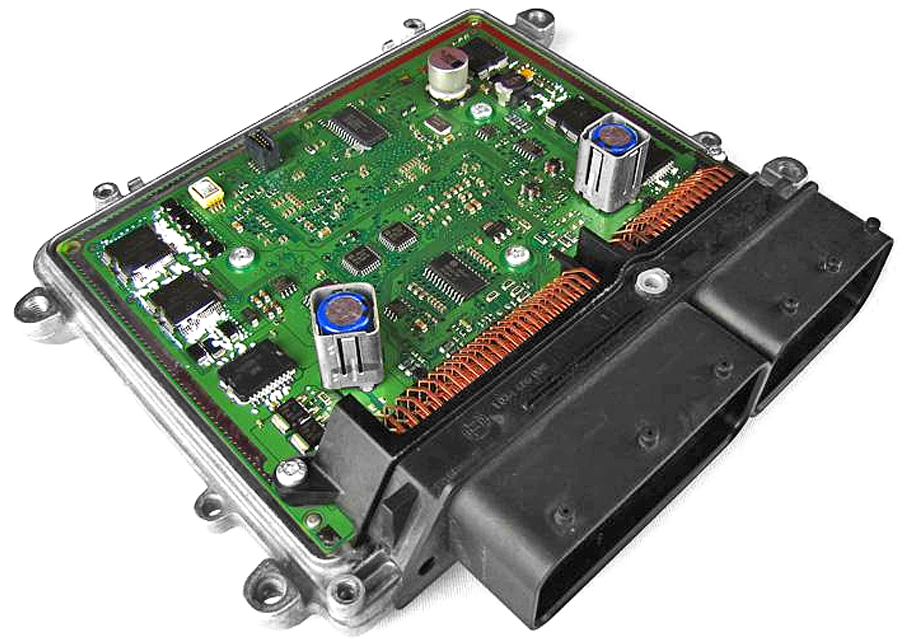
\includegraphics[width=0.45\textwidth]{cap2_ecu_board.png}}
	Adaptado de: \citeonline{EletroEmb}.
	\label{fig:cap2_ecu_image}
\end{figure}

As quantidade de entradas e saídas disponíveis está associada ao microprocessador/microcontrolador utilizado, e estas podem ser digitais ou analógicas, sendo que as saídas também podem ser do tipo \criarSigla[Driver do Lado Inferior]{Low Side Driver}{LSD} ou \criarSigla[Driver do Lado Superior]{High Side Driver}{HSD}.

Em um veículo, existem diversas ECUs, ligadas por uma ou mais redes CAN \emph{bus}. Dependendo da quantidade e distribuição no veículo, podem ser que diversas ECUs pertençam a um mesmo domínio e que uma delas sirva como uma central para as demais, ou ainda que uma ECU seja responsável por repassar informações de uma rede CAN para outra.

Como cada ECU deverá executar um algoritmo específico, o qual varia conforme a função para a qual a mesma foi designada, surge a necessidade de que haja um gerenciamento dos vários módulos espalhados pelo veículo. Esta responsabilidade cai em uma das ECUs, a qual faz uso de um sistema operacional padronizado, que é capaz de se comunicar com as demais unidades de maneira intermitente e que dê prioridade para recursos de maior importância.

\section{Padrões de Desenvolvimento de Software Automotivo}

Com o crescente uso de componentes eletrônicos embarcados nos veículos automotivos, também surgiu a necessidade de padronizar as etapas do desenvolvimento de novos sistemas, afim de garantir a interoperabilidade e a intercambialidade entre eles.

Serão apresentados aqui um padrão relacionado a engenharia de software e outro dedicado a implementação de sistemas veiculares.

\subsection{Modelo V}

Segundo \citeonline{ModelV}, o Modelo V, ou modelo de Verificação e Validação, pode ser considerado uma extensão do modelo Cascata, onde cada etapa deve ser concluída antes de avançar para a próxima. Ao invés de se deslocar para baixo de maneira linear, os passos do processo são curvados para cima após concluida a fase de codificação, tomando formato de um V, conforme ilustra a \reffig{cap2_development_modelv}.

\figura{cap2_development_modelv}{Modelo V}{8.5cm}{development_modelv}

Como vantagens, trata-se de um modelo de fácil utilização, que incentiva a criação de cenários de testes antes mesmo da produção do código. Permite também que defeitos sejam encontrados em fases iniciais e apresenta bom resultados em projetos de pequeno porte.

Entre suas desvantagens, pode-se destacar que trata-se de um modelo pouco flexível. A produção de código só tem seu início na fase de implementação, tornando impraticável a criação de um protótipo.

\subsection{OSEK/VDX}

Conforme \citeonline{OsekVdx}, o padrão OSEK/VDX foi idealizado como uma arquitetura aberta para ECUs veiculares. Ele surgiu a partir da união do padrões OSEK\footnote{\textbf{O}ffene \textbf{S}ysteme und deren Schnittstellen für die \textbf{E}lektronik in \textbf{K}raftfahrzeugen}, criado por um consórcio de fabricantes de veículos alemãs, com o padrão VDX\footnote{\textbf{V}ehicle \textbf{D}istributed e\textbf{X}ecutive}, criado pelas empresas francesas Renault e Peugeot. 

A principal motivação para a criação deste padrão se decorreu por conta do número cada vez maior de sistema eletrônicos nos veículos. Com a introdução do padrão, problemas recorrentes puderam ser corrigidos, como a imcompatibilidade entre ECUs de diferentes fabricantes, bem como a contenção de custos com o desenvolvimento de protocolos para as ECUs.

O padrão utiliza uma abordagem estática para as configurações do sistema, forçando com que todas as configurações sejam definidas antes da inicialização do sistema. Isto impede que novas tarefas sejam criadas ou que a memória seja alocada dinamicamente durante a execução do programa.

Para auxiliar na definição destas configurações, o padrão OSEK/VDX utiliza um arquivo de configuração com uma linguagem própria, chamada de \criarSigla[Linguagem de Implementação do OSEK]{OSEK Implementation Language}{OIL}. Uma vez definido, o arquivo é então processado para gerar o código em C de configuração do \criarSigla[Sistema Operacional de Tempo-Real]{Real Time Operating Systems}{RTOS}. A \reffig{cap2_development_osekvdx_oil} provê uma ilustração do processo de geração envolvendo o arquivo de configuração OIL.

\figura{cap2_development_osekvdx_oil}{Processo de geração do código em C a partir de um arquivo OIL}{\textwidth}{OsekOil}

O padrão conta com sete especificações, cada qual atendendo a uma área diferente do sistema, sendo elas:

\begin{itemize}
	\item \textbf{OSEK OS}: Sistema operacional;
	\item \textbf{OSEK Time}: Sistema operacional ativado por tempo;
	\item \textbf{OSEK COM}: Serviços de comunicação;
	\item \textbf{OSEK FTCOM}: Comunicação com tolerância a falhas;
	\item \textbf{OSEK NM}: Gerenciamento de rede;
	\item \textbf{OSEK OIL}: Configuração do kernel;
	\item \textbf{OSEK ORTI}: Configuração do kernel com suporte a debuggers;
\end{itemize}

Por ser um padrão mais antigo e restrito, atualmente existem soluções comerciais de código aberto, dentre elas: FreeOSEK\footnote{https://github.com/ciaa/Firmware/}, ERIKA Enterprise\footnote{http://erika.tuxfamily.org/drupal/} e Trampoline\footnote{http://trampoline.rts-software.org/}.

\subsection{AUTOSAR}

Confome \citeonline{AUTOSAR:HOME}, o projeto AUTOSAR surgiu da cooperação entre manufaturadores e fornecedores de veículos e industrias de componentes eletrônicos e de software. Desde sua concepção, em 2003, foi idealizado como um projeto aberto, focado na padronização de arquiteturas de software para a industria automotiva. O AUTOSAR também incorpora a maior parte do OSEK/VDX, expandindo suas funcionalidades mas mantendo a compatibilidade.

A motivação por trás do desenvolvimento do padrão AUTOSAR visava atender as otimizações a nível de sistema, e não apenas em componentes individuais, obtendo assim a máxima reutilização de código possível. Para tal, uma arquitetura aberta, escalar e de módulos de software intercambiáveis era necessária, exigindo um esforço coletivo do consórcio de empresas envolvidas.

O principal objetivo do AUTOSAR é a padronização de funções básicas de sistemas e interfaces funcionais, garantindo a integração, intercambialidade e transferência de funcionalidades em uma rede veicular entre os parceiros de desenvolvimento, além de permitir que novas aplicações sejam agregadas durante o ciclo de vida do veículo.

%O escopo da norma agrega todas as áreas de domínio eletrônico de um veículo automotivo, mas dá especial destaque para os domínios de trem de força, chassi e corpo do veículo.

Para cumprir seus objetivos técnicos de prover uma infraestrutura comum de software para sistemas automotivos, quatro características foram tidas como essenciais, sendo elas:

\begin{itemize}
	\item \textbf{Modularidade}: permite que pedaços de código sejam agregados conforme requerimento do software;
	\item \textbf{Escalabilidade}: promove a adaptação de módulos de software comuns para diferentes veículos;
	\item \textbf{Transferibilidade}: otimiza o uso de recursos disponíveis através da arquitetura eletrônica de um veículo;
	\item \textbf{Reusabilidade}: aumenta a qualidade do produto, utilizando códigos já testados;
\end{itemize}

Com base nestes conceitos, a arquitetura básica pode ser ilustrada na \reffig{cap2_autosar_modules}. Ela também demonstra como os módulos do AUTOSAR estão associados.

\figura{cap2_autosar_modules}{Visão geral técnica do AUTOSAR}{\textwidth}{AUTOSAR:HOME}
